% HiMCM 2019 Problem A --- Airport terminal charging (BDI--DES study pack)
% Compile from paper/:
%   pdflatex himcm_paper.tex && bibtex himcm_paper && pdflatex himcm_paper.tex && pdflatex himcm_paper.tex
% All numeric cells are copied from ../results/*.csv. No invented statistics.
% Writing style target: ~80% ASD-STE100 (one fact per sentence; <=25 words).
\documentclass[11pt]{article}

\usepackage[margin=1in]{geometry}
\usepackage{amsmath,amssymb}
\usepackage{booktabs}
\usepackage{graphicx}
\usepackage{caption}
\usepackage{setspace}
\usepackage{array}
\usepackage{enumitem}
\usepackage[hidelinks]{hyperref}

\graphicspath{{../paper_figures/}{paper_figures/}{./}}
\hypersetup{
  pdftitle={HiMCM 2019 Problem A: Terminal Charging Kiosk Design},
  pdfauthor={GoHiMCM 2019 A study team}
}

\newcommand{\TeamNumber}{GoHiMCM}

\pagestyle{myheadings}
\markright{\TeamNumber \hfill HiMCM 2019 Problem A \hfill}

\title{\textbf{BDI Passenger Agents in a SimPy Charging Sandbox:\\
Pareto Kiosk Sizing under Thunderstorm Delay}\\[0.35em]
\large HiMCM 2019 Problem A --- Team \TeamNumber}
\author{}
\date{}

\begin{document}
\maketitle
\thispagestyle{empty}

\noindent
Companion files: \texttt{summary\_sheet.tex} (one page),
\texttt{airport\_authority\_letter.tex} (operations brief),
\texttt{ai\_disclosure.tex} (COMAP AI report).
All tables and figures read locked files under \texttt{results/}
and \texttt{paper\_figures/}.

\tableofcontents
\newpage

%======================================================================
\section{Introduction and micro-cognitive formulation}
%======================================================================

Airports sell boarding time and phone battery at the same desk.
A dead phone raises missed-connection risk and service complaints.
We size charging kiosks under CapEx and floor-area caps.

We model each traveler as a \textbf{BDI passenger agent}
(Belief--Desire--Intention)~\cite{bdi2026}.
Beliefs hold battery state of charge (SOC) and minutes to boarding
$T_{\mathrm{board}}$.
Desires encode ``stay connected until gate call.''
Intentions select a charging kiosk, wait, rent a power bank, or abort.

Empirical priors in our code are fixed and auditable.
About $25\%$ of arrivals start anxious about low SOC.
Boarding slack is drawn as $T_{\mathrm{board}}\sim U(45,120)$ minutes.
Utility $U_{\mathrm{charge}}$ rejects any plan that risks a missed flight.

The agent state machine is
\[
\mathrm{IDLE}\to\mathrm{SEEK}\to\mathrm{QUEUE}
\to\{\mathrm{CHARGE},\mathrm{RENT},\mathrm{RENEGING},\mathrm{ABORT}\}.
\]
Reneging probability rises when $T_{\mathrm{board}}$ is short and the
wait queue is long.
Unit test: if $T_{\mathrm{board}}=10$ and queue length $>5$,
reneging probability equals $1$.

\paragraph{Design questions.}
How many fast kiosks, slow lockers, and power-bank banks should we buy?
What CapEx--wait trade-off is non-dominated?
How does a 17:00 thunderstorm delay shock change reneging probability?

\paragraph{Caps (locked).}
Budget $\le \$80{,}000$.
Area $\le 40\,\mathrm{m}^2$.
A fast kiosk costs $\$2{,}000$.
A slow locker costs $\$1{,}200$.
A power-bank bank costs $\$3{,}500$.
Unit areas are $0.8$, $2.0$, and $0.5\,\mathrm{m}^2$.


%======================================================================
\section{SimPy discrete-event queueing sandbox and control-flow mapping}
%======================================================================

We embed each BDI passenger agent in a SimPy process
(\texttt{src/des\_env/airport\_sim.py}).
Three resource pools map to hardware:
$C_{\mathrm{fast}}$ (65\,W fast kiosk),
$C_{\mathrm{slow}}$ (15\,W locker),
$C_{\mathrm{bank}}$ (power-bank rental).

Arrivals follow a non-homogeneous Poisson process over $16$ hours
($06{:}00$--$22{:}00$).
Intensity $\lambda(t)$ has three daily peaks.
Default normal day: $\lambda_{\mathrm{base}}=0.35$, peak multiplier $3$.
Morning-rush densify runs use $\lambda_{\mathrm{base}}=0.55$, multiplier $4$.

Figure~\ref{fig:stage2} shows a Stage-2 baseline day with pack
$(C_{\mathrm{fast}},C_{\mathrm{slow}},C_{\mathrm{bank}})=(12,15,2)$.
Table~\ref{tab:stage2} lists locked KPIs from
\texttt{stage2\_baseline\_metrics.csv}.
Mean wait time is $0.00$ minutes.
Reneging probability is $0.00$.
Fast-kiosk utilization is $5.72\%$.
Slow-locker utilization is $24.24\%$.
$n=441$ arrivals; $110$ anxious seekers.

\begin{figure}[htbp]
  \centering
  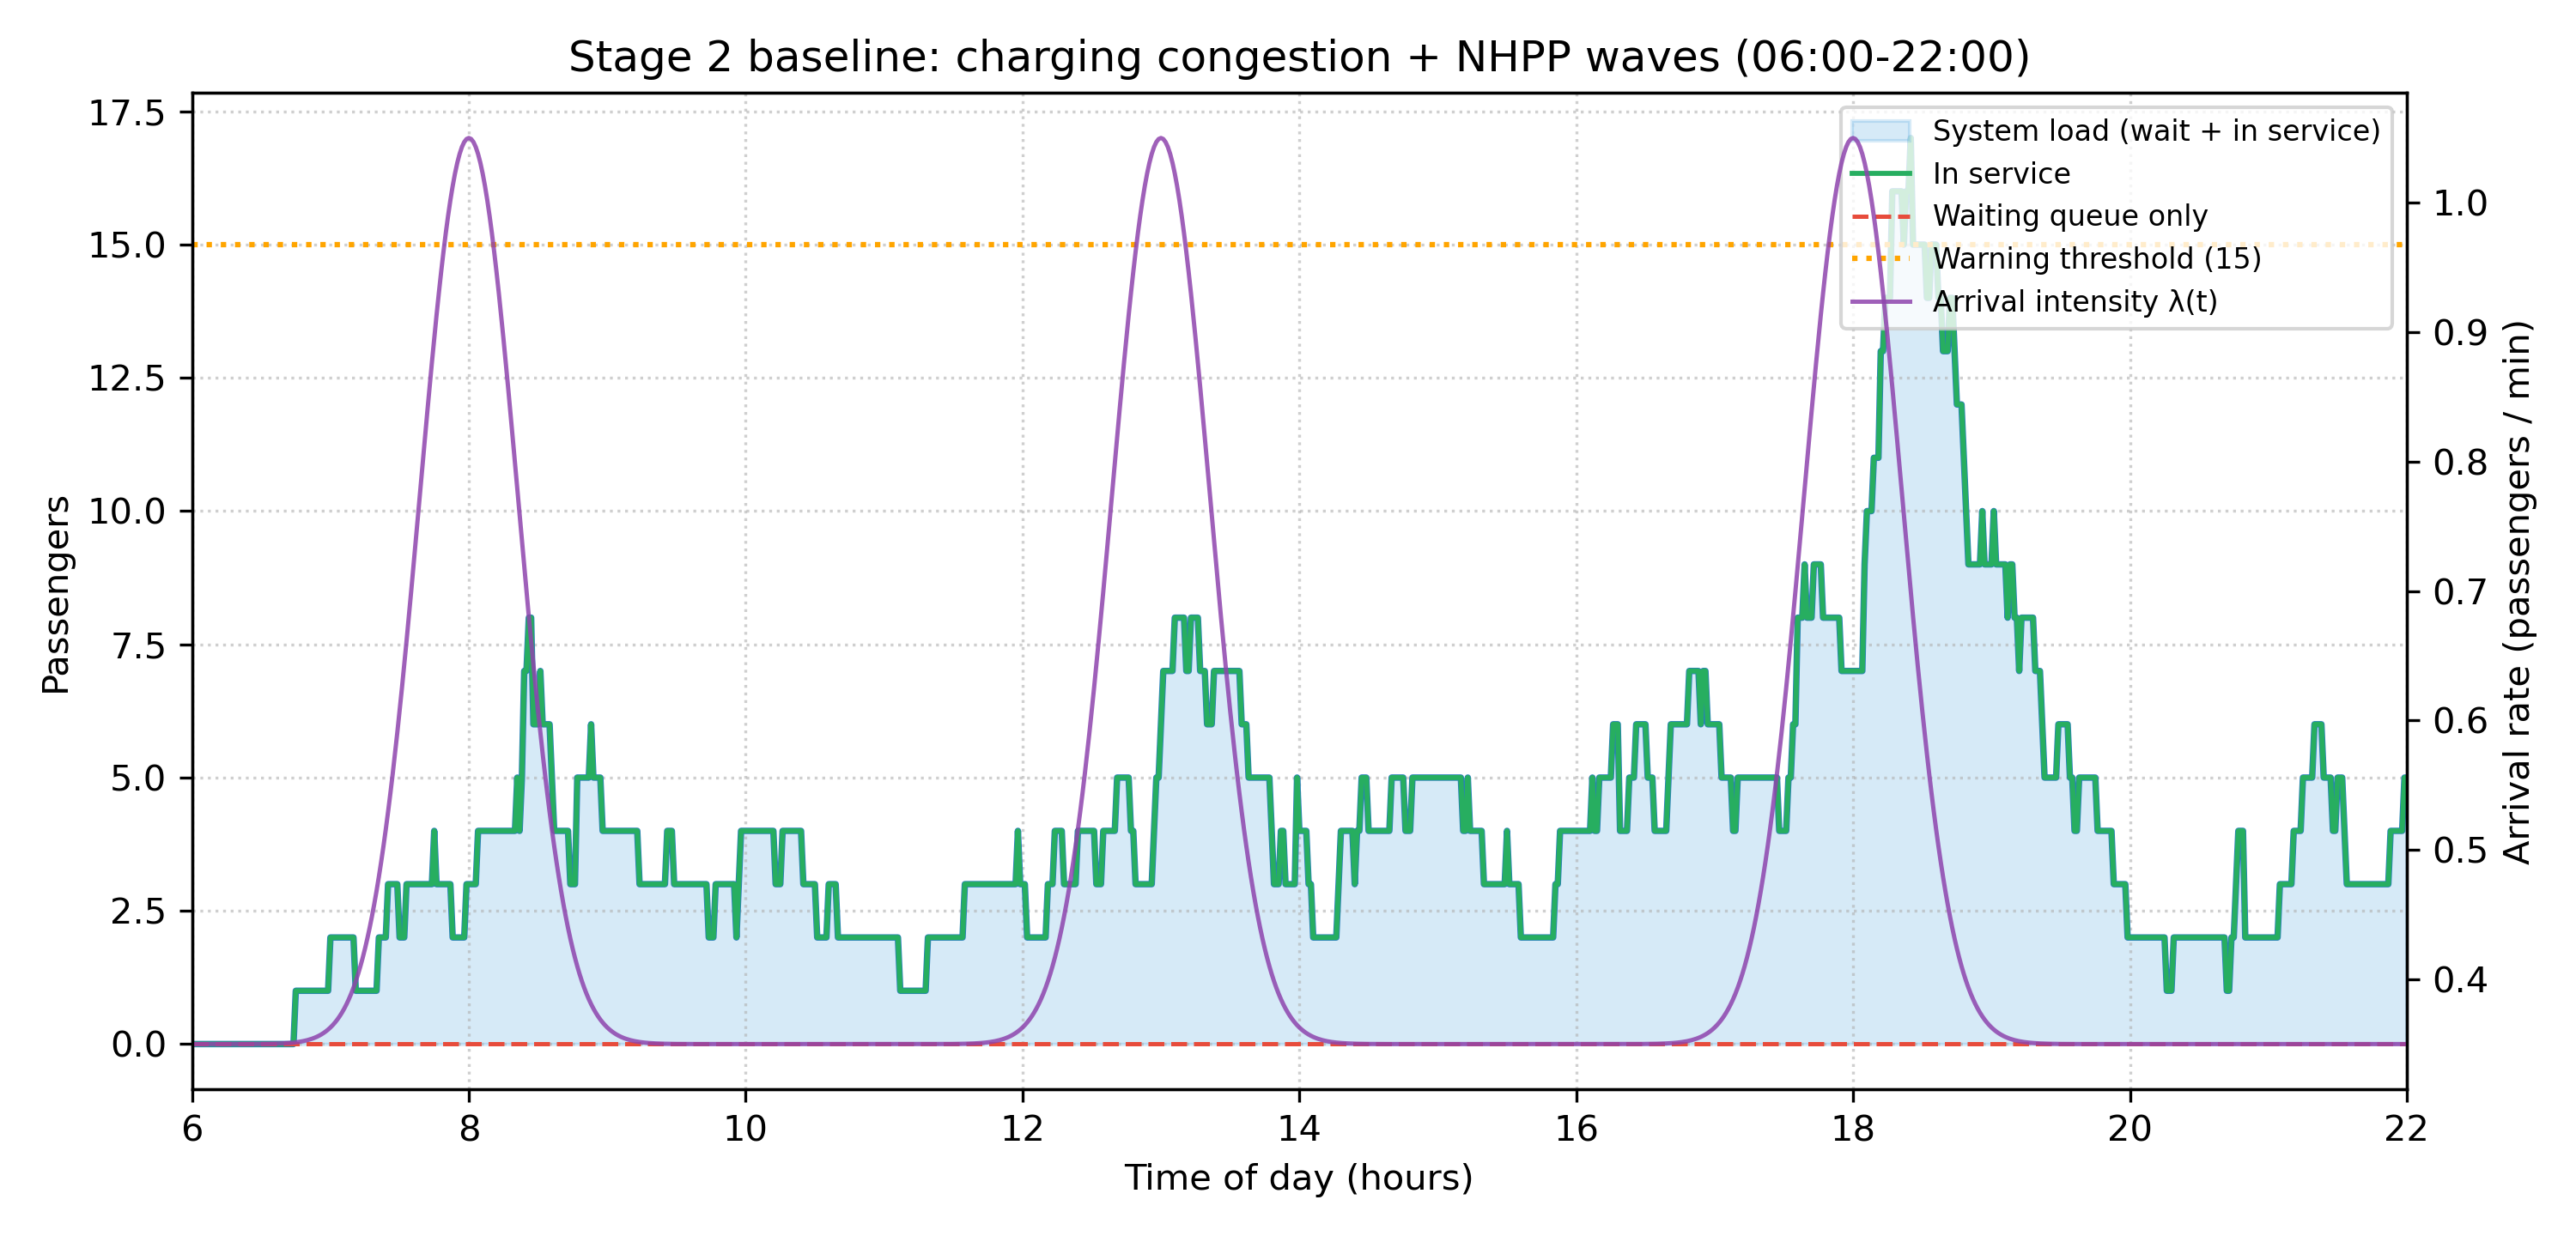
\includegraphics[width=0.92\textwidth]{stage2_queue_baseline.png}
  \caption{Stage-2 baseline load and intensity ($12/15/2$, normal day).
  Source: \texttt{paper\_figures/stage2\_queue\_baseline.png}.}
  \label{fig:stage2}
\end{figure}

\begin{table}[htbp]
\centering
\caption{Stage-2 baseline KPIs. Source: \texttt{stage2\_baseline\_metrics.csv}.}
\label{tab:stage2}
\begin{tabular}{lrr}
\toprule
Metric & Symbol / field & Value \\
\midrule
Arrivals & \texttt{total\_passengers} & $441$ \\
Anxious seekers & \texttt{anxious\_passengers} & $110$ \\
Served at fast kiosk & \texttt{served\_fast} & $37$ \\
Served at slow locker & \texttt{served\_slow} & $73$ \\
Power-bank rentals & \texttt{served\_powerbank} & $0$ \\
Mean wait (min) & \texttt{mean\_wait\_time} & $0.00$ \\
Reneging probability & \texttt{reneging\_rate} & $0.00$ \\
Max system load & \texttt{max\_system\_load} & $17$ \\
Util.\ fast / slow & utilization & $0.057$ / $0.242$ \\
\bottomrule
\end{tabular}
\end{table}

\paragraph{Control-flow mapping.}
\texttt{passenger\_process} requests a resource, waits, then charges or rents.
Boarding deadline forces early release of the charging kiosk.
Telemetry records queue length, system load, and intention flows.

\paragraph{Storm injection (preview).}
At $t=660$ minutes ($17{:}00$), $40\%$ of later departures gain
$2$--$4$ hours of delay.
SOC drain doubles for delayed BDI passenger agents.
Section~\ref{sec:stress} reports the stress KPIs.


%======================================================================
\section{FastMCP protocol and LangGraph self-reflection agent}
%======================================================================

Agents must call the sandbox without rewriting SimPy internals.
We wrap the DES as a FastMCP server
(\texttt{src/mcp\_server/server.py}).

\paragraph{Tools.}
\texttt{run\_charging\_simulation} runs one day and returns KPIs.
\texttt{validate\_infrastructure\_budget} checks CapEx and area caps.
Resource \texttt{config://airport\_constraints} publishes unit costs.

\paragraph{LangGraph loop.}
The reflection agent
(\texttt{src/des\_agent/reflection\_agent.py}) runs
\[
\mathrm{propose}\to\mathrm{validate}\to\mathrm{simulate}
\to\mathrm{reflect}\to\mathrm{check}.
\]
A local Ollama model (\texttt{qwen2.5:7b}) drafts the next pack.
If Ollama is offline, a deterministic rule proposer continues.
Budget rejection is limited to three retries per iteration.

\paragraph{Acceptance targets.}
Mean wait $\le 5$ minutes.
Reneging probability $\le 0.05$.
Traces are stored under \texttt{results/reflection\_*.json}.

This loop is the micro-search engine for Section~\ref{sec:pareto}.
It does not invent CSV rows.
Every accepted candidate is a real DES call.


%======================================================================
\section{Dual-LLM autonomous planning and empirical Pareto sizing}
\label{sec:pareto}
%======================================================================

A planning agent splits the CapEx problem into four subtasks
(\texttt{planning\_agent.py}).
Subtask budgets are $\$40{,}000$, $\$80{,}000$, pricing free-window,
and pricing full-metered.
Each subtask calls the reflection loop.
Summary file: \texttt{autonomous\_planning\_summary.json}
(\texttt{plan\_source=ollama}).

Table~\ref{tab:plan} lists locked subtask outcomes.
Pack $4/0/3$ meets a low CapEx but shows reneging probability $0.637$.
That pack is not service-feasible for kiosk sizing.

\begin{table}[htbp]
\centering
\caption{Autonomous planning candidates.
Source: \texttt{autonomous\_planning\_summary.json}.}
\label{tab:plan}
\begin{tabular}{llrrr}
\toprule
ID & Pack $(C_f,C_s,C_b)$ & CapEx (USD) & Wait (min) & Reneging \\
\midrule
001 & $8/10/3$ & $38{,}500$ & $0.163$ & $0.000$ \\
002 & $15/10/8$ & $70{,}000$ & $0.163$ & $0.000$ \\
003 & $4/0/3$ & $18{,}500$ & $0.000$ & $0.637$ \\
004 & $20/10/8$ & $80{,}000$ & $0.163$ & $0.000$ \\
\bottomrule
\end{tabular}
\end{table}

\paragraph{Pareto construction.}
We re-simulate planning packs under rush intensity.
We densify a feasible hardware grid (216 unique packs).
Objectives:
\[
\min \mathrm{CapEx},\qquad \min \overline{W}.
\]
We keep only packs with reneging probability $\le 0.05$.
We extract the non-dominated front
(\texttt{optimal\_kiosk\_sizing.csv}).

Table~\ref{tab:pareto} lists the seven Pareto points.
The recommended knee sits under the $\$80{,}000$ CapEx line.
The knee pack is $(C_{\mathrm{fast}},C_{\mathrm{slow}},C_{\mathrm{bank}})=(8,16,0)$.
CapEx is $\$35{,}200$.
That CapEx uses $44\%$ of the CapEx cap.
Area is $38.4\,\mathrm{m}^2$.
Rush mean wait is $0.0115$ minutes.
Rush reneging probability is $0.00$.

The cheapest Pareto pack is $4/8/0$ with wait $5.91$ min.
Moving to the knee cuts mean wait by $99.8\%$.
Extra CapEx beyond $\$35{,}200$ does not reduce wait on this front.

\begin{table}[htbp]
\centering
\caption{Pareto front (reneging $\le 5\%$).
Source: \texttt{optimal\_kiosk\_sizing.csv}.}
\label{tab:pareto}
\begin{tabular}{rrrrrr}
\toprule
$C_f$ & $C_s$ & $C_b$ & CapEx & Wait (min) & Reneging \\
\midrule
4 & 8 & 0 & $17{,}600$ & $5.909$ & $0.046$ \\
2 & 12 & 0 & $18{,}400$ & $3.575$ & $0.020$ \\
4 & 12 & 0 & $22{,}400$ & $1.466$ & $0.010$ \\
6 & 12 & 0 & $26{,}400$ & $1.258$ & $0.010$ \\
4 & 16 & 0 & $27{,}200$ & $1.038$ & $0.000$ \\
6 & 16 & 0 & $31{,}200$ & $0.124$ & $0.000$ \\
8 & 16 & 0 & $35{,}200$ & $0.011$ & $0.000$ \\
\bottomrule
\end{tabular}
\end{table}

\begin{figure}[htbp]
  \centering
  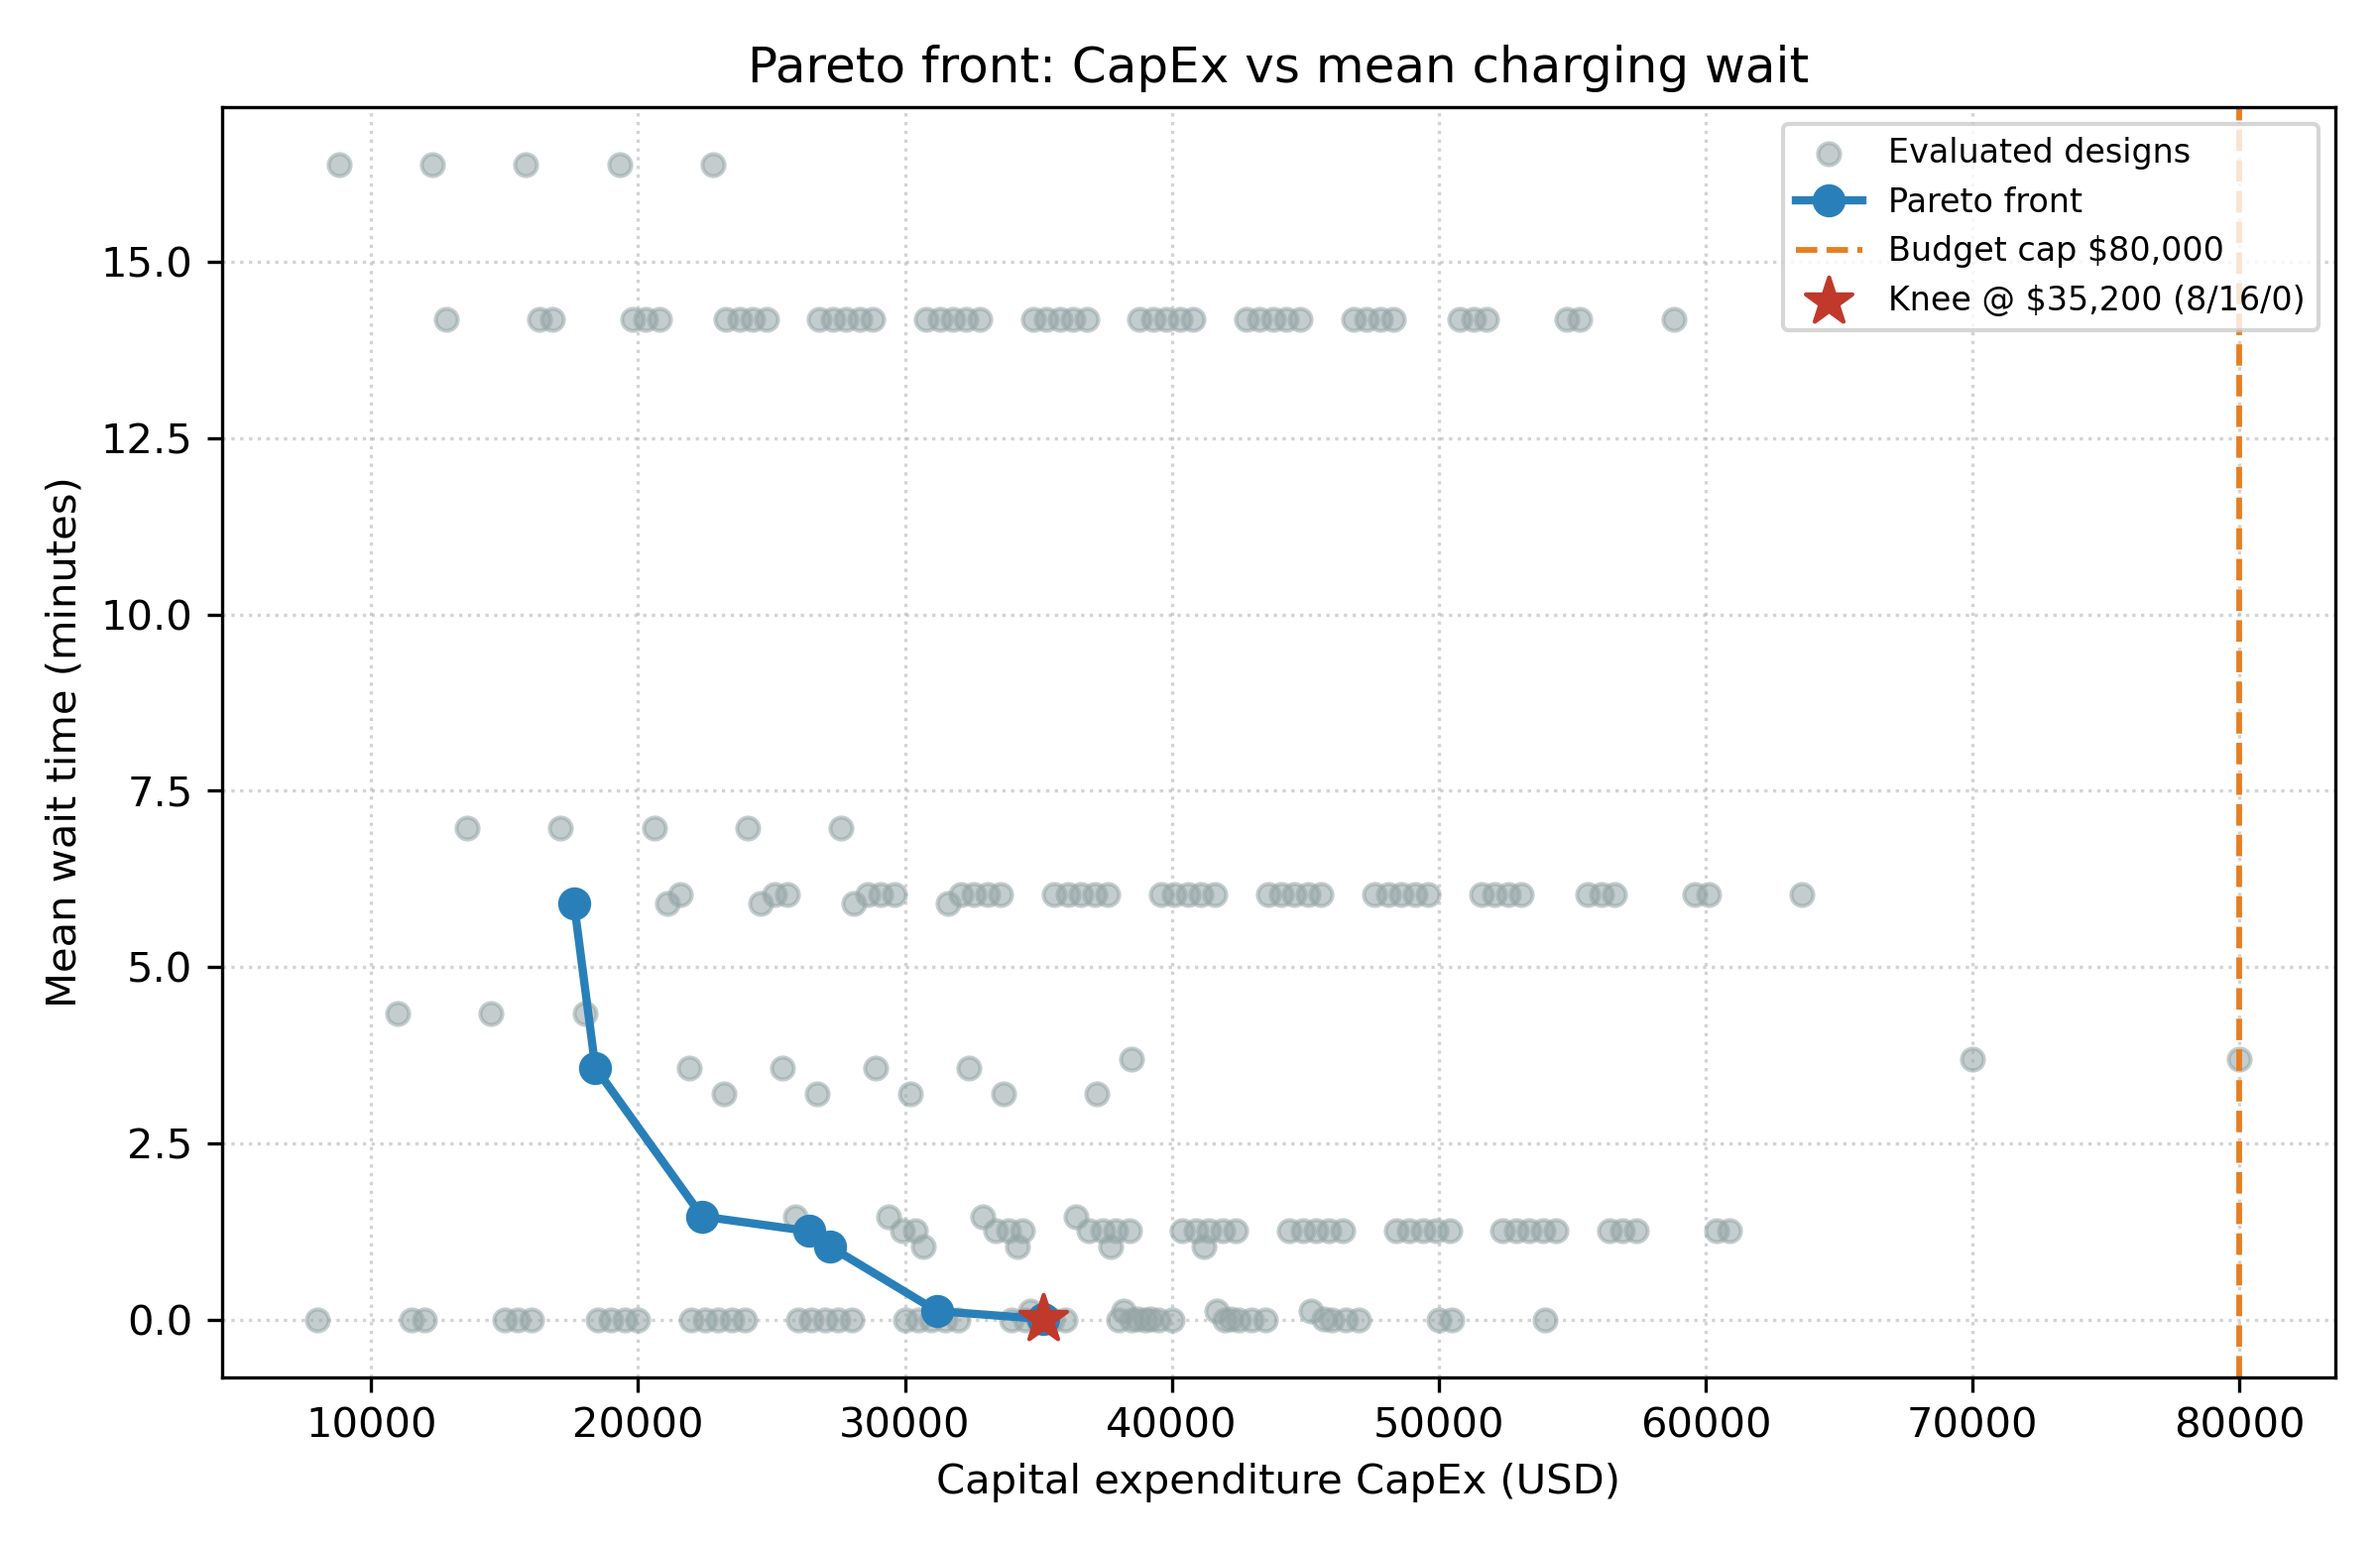
\includegraphics[width=0.88\textwidth]{fig_pareto_cost_vs_wait.png}
  \caption{CapEx versus mean wait with $\$80{,}000$ budget line and knee.
  Source: \texttt{fig\_pareto\_cost\_vs\_wait.png}.}
  \label{fig:pareto}
\end{figure}


%======================================================================
\section{Cascading flight delay stress testing and resilience}
\label{sec:stress}
%======================================================================

We inject a thunderstorm delay at $17{:}00$.
$40\%$ of later departures receive $2$--$4$ hours of added delay.
Delayed BDI passenger agents double SOC drain.
$n=621$ arrivals share one random seed across packs.

We compare empirical pack $12/15/2$ (CapEx $\$49{,}000$)
to the Pareto knee $8/16/0$ (CapEx $\$35{,}200$).
Table~\ref{tab:stress} copies
\texttt{thunderstorm\_stress\_comparison.csv}.

\begin{table}[htbp]
\centering
\caption{Thunderstorm stress KPIs (shared seed).
Source: \texttt{thunderstorm\_stress\_comparison.csv}.}
\label{tab:stress}
\begin{tabular}{lrr}
\toprule
KPI & Baseline $12/15/2$ & Knee $8/16/0$ \\
\midrule
CapEx (USD) & $49{,}000$ & $35{,}200$ \\
Mean wait (min) & $4.591$ & $2.347$ \\
Reneging probability & $0.0229$ & $0.0114$ \\
Max wait-queue length & $6$ & $6$ \\
Max system load & $23$ & $24$ \\
Storm-delayed agents & $155$ & $165$ \\
Arrivals & $621$ & $621$ \\
\bottomrule
\end{tabular}
\end{table}

\paragraph{Resilience deltas (locked).}
Mean wait falls by $48.9\%$ ($4.591\to 2.347$ min).
Reneging probability falls by $50.3\%$ ($0.0229\to 0.0114$).
CapEx falls by $28.2\%$ versus the empirical pack.
Peak wait-queue length stays at $6$ for both packs.

Figure~\ref{fig:stress} plots $16$-hour load with a red storm window.
Figure~\ref{fig:sankey} shows BDI intention splits under the same shock.
Anxious seekers divert among fast kiosk, slow locker, power bank, and abort.

\begin{figure}[htbp]
  \centering
  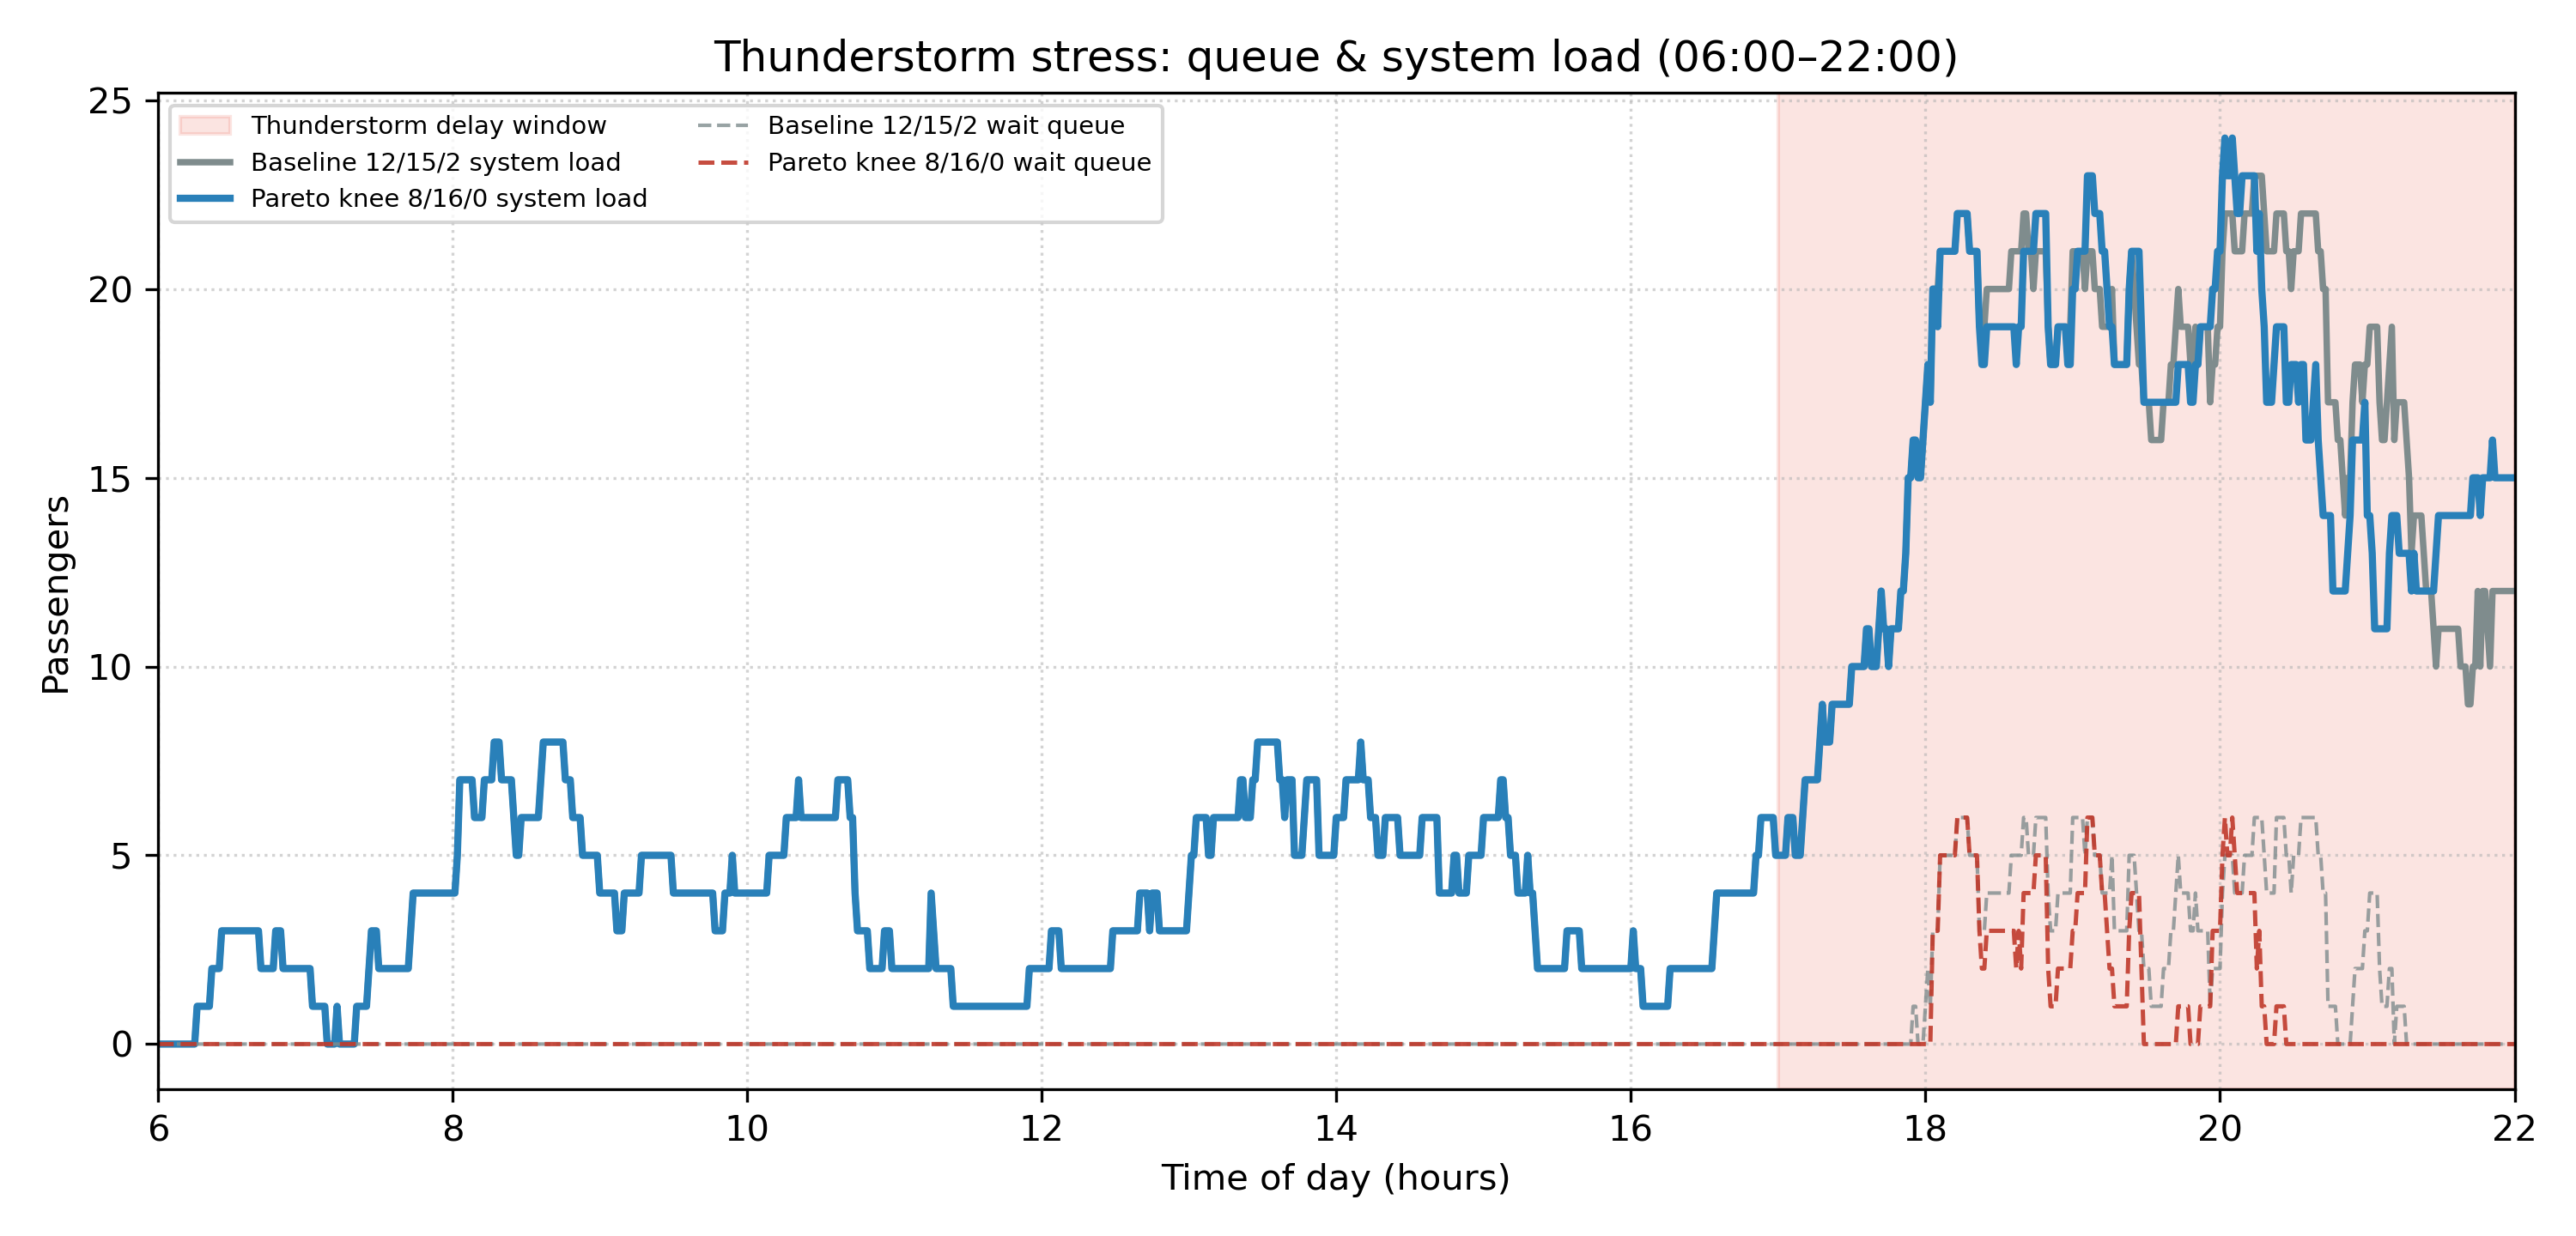
\includegraphics[width=0.95\textwidth]{fig_queue_length_delay_stress.png}
  \caption{System load and wait queue under thunderstorm delay.
  Source: \texttt{fig\_queue\_length\_delay\_stress.png}.}
  \label{fig:stress}
\end{figure}

\begin{figure}[htbp]
  \centering
  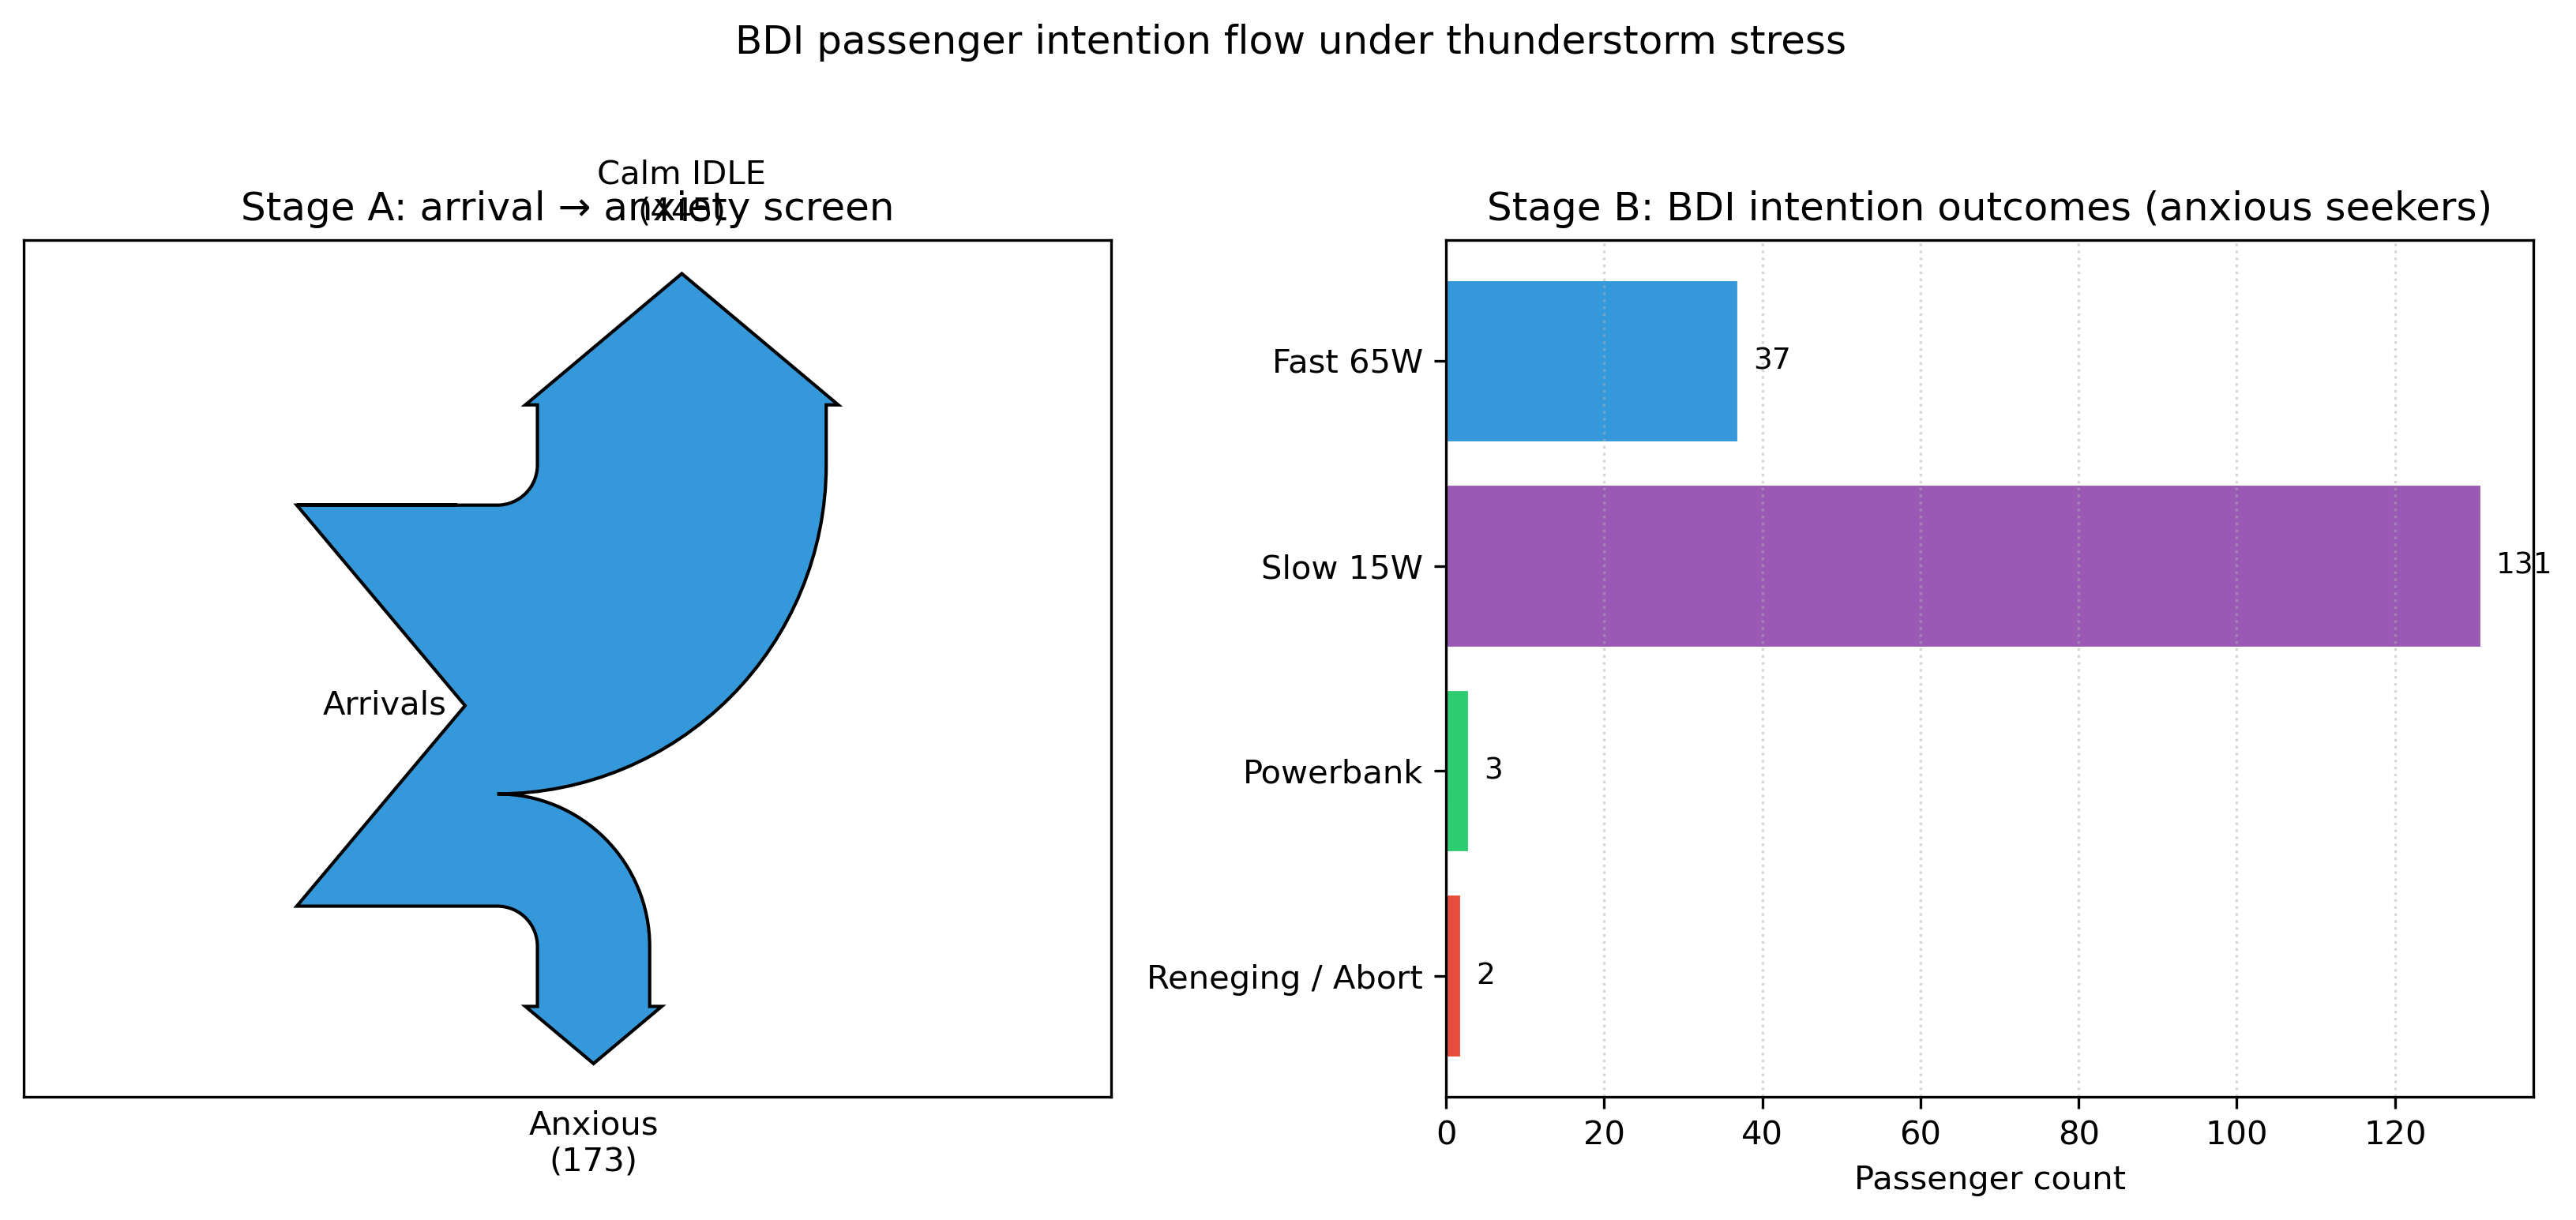
\includegraphics[width=0.92\textwidth]{fig_bdi_intention_flow_sankey.png}
  \caption{BDI passenger agent intention flow under storm stress.
  Source: \texttt{fig\_bdi\_intention\_flow\_sankey.png}.}
  \label{fig:sankey}
\end{figure}

\paragraph{Operational reading.}
More fast kiosks alone do not buy resilience.
The knee keeps sixteen slow lockers and zero power-bank banks.
Under this seed, slow capacity absorbs stranded dwell better than
the heavier empirical mix.


%======================================================================
\section{Strengths and limitations}
%======================================================================

\paragraph{Strengths.}
\begin{enumerate}[leftmargin=1.4em,itemsep=0.2em]
  \item Every KPI cites a locked CSV path under \texttt{results/}.
  \item BDI passenger agents couple SOC, boarding slack, and reneging.
  \item FastMCP + LangGraph make DES calls tool-shaped and auditable.
  \item Pareto filter enforces reneging probability $\le 0.05$.
  \item Storm test uses one seed for fair pack comparison.
\end{enumerate}

\paragraph{Limitations.}
\begin{enumerate}[leftmargin=1.4em,itemsep=0.2em]
  \item Arrival intensity is synthetic NHPP, not airport AODB feeds.
  \item Gate geography is not a spatial queueing network.
  \item Power-bank banks are zero on the current knee; inventory risk
        is not priced.
  \item Ollama drafts proposals; offline mode falls back to rules.
  \item One storm seed is not a full Monte Carlo envelope.
\end{enumerate}

\paragraph{Recommendation.}
Deploy pack $8/16/0$ first ($\$35{,}200$, $38.4\,\mathrm{m}^2$).
Keep CapEx headroom under $\$80{,}000$ for gate-cluster add-ons.
Re-run storm seeds before capital release.

\section*{References}
\begin{thebibliography}{9}
\bibitem{bdi2026}
BDI--DES passenger decision model (arXiv:2602.13878).
Local PDF: \texttt{data/raw/papers/arxiv\_2602.13878\_bdi\_des.pdf}.

\bibitem{simpy}
Team SimPy.
\textit{SimPy: Discrete-event simulation in Python}.
\url{https://simpy.readthedocs.io/}.

\bibitem{mcp}
Anthropic.
\textit{Model Context Protocol (MCP) specification}.
\url{https://modelcontextprotocol.io/}.

\bibitem{langgraph}
LangChain.
\textit{LangGraph}.
\url{https://langchain-ai.github.io/langgraph/}.
\end{thebibliography}

\end{document}
